\documentclass[11pt,a4paper, twocolumn]{article}
\usepackage{float}
\usepackage{verbatim}
\usepackage{subfig}
\usepackage[T1]{fontenc}
\usepackage[utf8]{inputenc}
\usepackage{geometry}
\geometry{verbose,lmargin=1cm,rmargin=1cm, bmargin=2cm, tmargin=2cm}
\usepackage{enumitem}
\usepackage{calc}
\usepackage{wrapfig}
\usepackage{graphicx}
\usepackage{amssymb}
\usepackage{amsmath}
\usepackage{esint}
\usepackage{blindtext}
\usepackage{hyperref}
\usepackage{listings}

\hypersetup{
    colorlinks=true,
    linkcolor=blue,
    filecolor=magenta,
    urlcolor=cyan,
}
\usepackage{listings}
\lstset{ %
  backgroundcolor=\color{white},   % choose the background color; you must add \usepackage{color} or \usepackage{xcolor}; should come as last argument
  basicstyle=\footnotesize,        % the size of the fonts that are used for the code
  breakatwhitespace=false,         % sets if automatic breaks should only happen at whitespace
  breaklines=true,                 % sets automatic line breaking
  captionpos=t,                    % sets the caption-position to bottom
  commentstyle=\color{teal},    % comment style
  deletekeywords={...},            % if you want to delete keywords from the given language
  escapeinside={\%*}{*)},          % if you want to add LaTeX within your code
  extendedchars=true,              % lets you use non-ASCII characters; for 8-bits encodings only, does not work with UTF-8
  frame=single,                    % adds a frame around the code
  keepspaces=true,                 % keeps spaces in text, useful for keeping indentation of code (possibly needs columns=flexible)
  keywordstyle=\color{blue},       % keyword style
 % language=Python,                 % the language of the code
  morekeywords={*,...},           % if you want to add more keywords to the set
  numbers=left,                    % where to put the line-numbers; possible values are (none, left, right)
  numbersep=5pt,                   % how far the line-numbers are from the code
  numberstyle=\tiny\color{black}, % the style that is used for the line-numbers
  rulecolor=\color{black},         % if not set, the frame-color may be changed on line-breaks within not-black text (e.g. comments (green here))
  showspaces=false,                % show spaces everywhere adding particular underscores; it overrides 'showstringspaces'
  showstringspaces=false,          % underline spaces within strings only
  showtabs=false,                  % show tabs within strings adding particular underscores
  stepnumber=1,                    % the step between two line-numbers. If it's 1, each line will be numbered
  tabsize=2,                       % sets default tabsize to 2 spaces
  title=\lstname                   % show the filename of files included with \lstinputlisting; also try caption instead of title
}
\begin{document}

\title{Project 1\\
\normalsize{FYS3150 - Computational Physics}\\}

\author{Nicholas Karlsen}


\date{\today}% It is always \today, today,
%  but any date may be explicitly specified

\twocolumn[
  \begin{@twocolumnfalse}
    \maketitle
    \begin{abstract}
      This is an abstract
    \end{abstract}
  \end{@twocolumnfalse}
]

%\tableofcontents

\section{Introduction \label{sect:intro}}

\section{Method \label{sect:method}}

  We have second order inhomogeneous differential equation, Eqn. \ref{differential_equation}
  \begin{equation}
    \label{differential_equation}
    \frac{d^2u(x)}{dx^2} = f(x)
  \end{equation}
  With boundary conditions $\ddot{u}(x) = f(x)$, $u(0) = u(1) = 0$ and $x \in (0, 1)$.

  If we let $f(x) = 100e^{-10x}$, then it can be shown analytically that the differential equation has a solution Eqn. \ref{diffeq anal sol}
  \begin{equation}
    \label{diffeq anal sol}
    u(x) = 1 - (1 - e^{-10})x - e^{-10x}
  \end{equation}

  This problem can also be solved numerically by discretization. By taylor expansion in the form Eqn. \ref{Discrete diffeq}
  \begin{equation}
    \label{Discrete diffeq}
    - \frac{v_{i+1} + v_{i-1} + 2v_i}{h^2} = f_i
  \end{equation}
  where $h = 1/(n+1)$ is the step size for $n+1$ points.

  This problem can be written in the form 
  \begin{equation}
    A\vec v = \vec b
  \end{equation}
  Where $\textup A \in R^{n \times n}$ is a tridiagonal matrix with diagonal elements 2 and -1 (Eqn. \ref{A matrix}) and $\vec b =h^2(f_1, \dots, f_n)$.
  \begin{equation}
    \label{A matrix}
    A = \left[ 
    \begin{matrix}
      2 & -1 & 0 & \dots  & \dots &0 \\
      -1 & 2 & -1 & 0 & \dots &  0 \\
      0 & -1 & 2 & -1 & \dots & \vdots  \\
      \vdots & \vdots & \vdots & \vdots & \vdots & -1\\
      \dots & \dots & \dots & \dots & -1 & 2
    \end{matrix}
    \right]
  \end{equation}

  By matrix multiplication, when we multiply   the $i$-th row of $A$ by $\vec v$, we get
  \begin{align}
  \begin{split}
 -1 v_{i -1} + 2v_i - 1v_{i+1}  &= -\left( v_{i+1} + v_{i-1} - 2v_i\right) 
                                \\&= h^2f_i
  \end{split}
  \end{align}

  Which is equivalent to the discretized differential equation Eqn. \ref{Discrete diffeq},
  showing that the differential equation can be solved as a linear algebra problem rather than iteratively.

  \subsection{Analysis}
    The algorithms which were outlined in section \ref{sect:method} were implemented in Python 2.7, and the all of the source code can be found on my github: \url{https://github.com/nicholaskarlsen/FYS3150}

    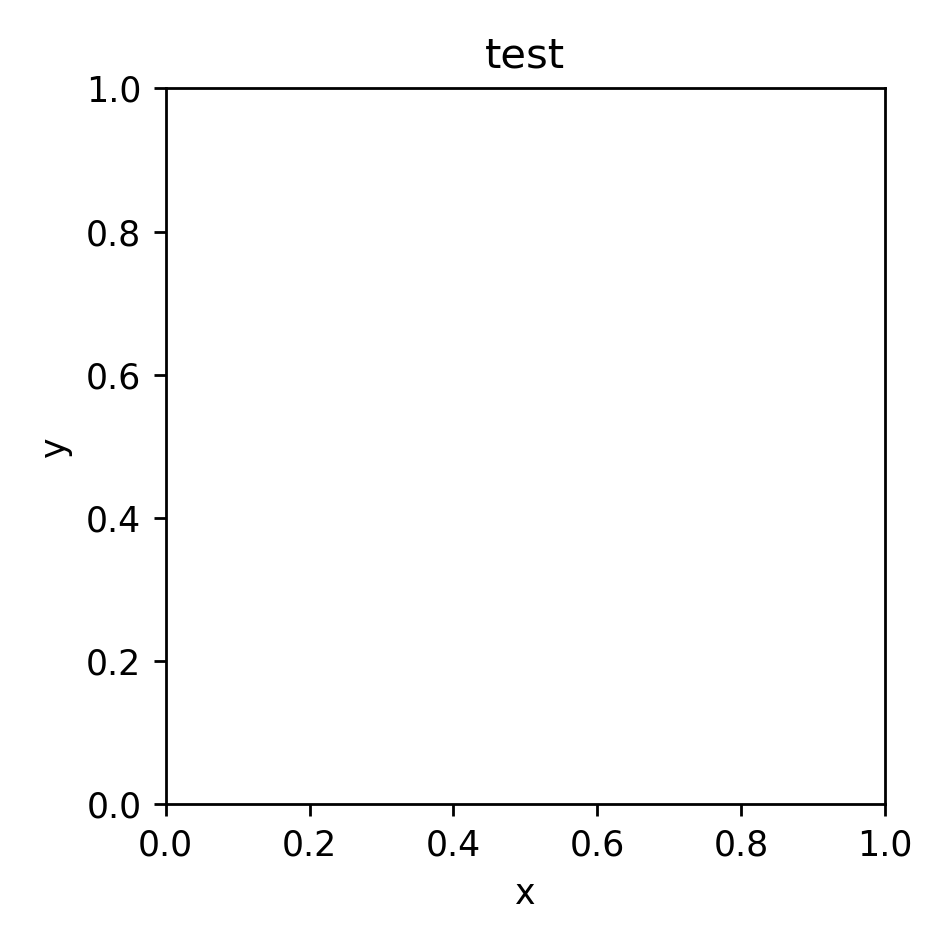
\includegraphics{figs/testfile.png}

  \subsection{Discussion}
%\appendix
%\section{Critique}

\end{document}